\documentclass[aspectratio=169]{beamer}
\usepackage[T1]{fontenc}
\usepackage[utf8]{inputenc}
\usepackage{lmodern}
\usepackage{graphicx}
\usepackage{amsmath,amssymb}
\usecolortheme{beaver}
\usefonttheme[onlymath]{serif}
\setbeamertemplate{navigation symbols}{}
\setbeamertemplate{footline}{}
\setbeamersize{text margin left=0.45cm,text margin right=0.45cm}
\setbeamerfont{frametitle}{size=\Large}
% Generated from results/*.csv by code/reporting.py
\newcommand{\ExperimentN}{180}
\newcommand{\ExperimentD}{6}
\newcommand{\ExperimentSeedCount}{5}
\newcommand{\ExperimentRunCount}{100}
\newcommand{\ExperimentRhoMax}{1}
\newcommand{\ExperimentSeconds}{66.4}
\newcommand{\EdgeMin}{2324}
\newcommand{\EdgeMax}{2474}
\newcommand{\DirParameterCount}{5825}
\newcommand{\ControlParameterCount}{5841}
\newcommand{\DirectedAUCMean}{0.723}
\newcommand{\DirectedAUCSD}{0.030}
\newcommand{\DirectedAPMean}{0.655}
\newcommand{\DirectedAPSD}{0.042}
\newcommand{\ControlAUCMean}{0.575}
\newcommand{\ControlAUCSD}{0.050}
\newcommand{\ControlAPMean}{0.559}
\newcommand{\ControlAPSD}{0.035}
\newcommand{\DeltaAUCMean}{0.148}
\newcommand{\DeltaAUCSD}{0.020}
\newcommand{\DeltaAPMean}{0.095}
\newcommand{\DeltaAPSD}{0.009}

\title{Edge orientation in link prediction}
\author{Nikita Scheglov}
\date{23 October 2026}

\begin{document}
\begin{frame}[t]{Edge orientation in link prediction}
\vspace{-0.15cm}
{\small\textbf{Idea:} aggregate incoming and outgoing neighbors separately.}
\vspace{0.05cm}

\begin{columns}[T,onlytextwidth]
\begin{column}{0.64\textwidth}
\centering
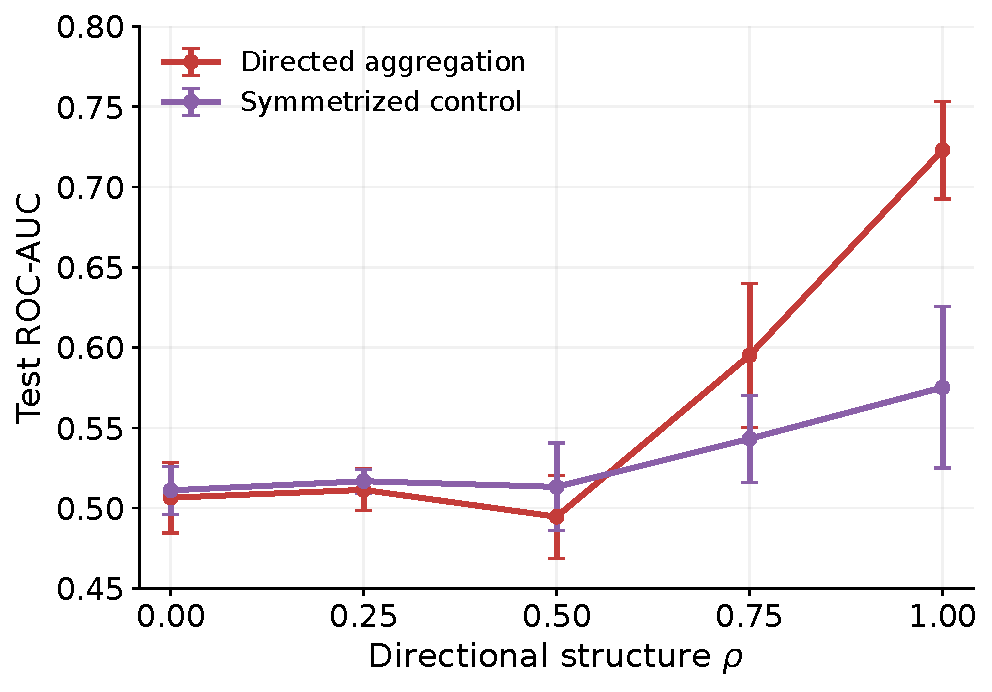
\includegraphics[width=\linewidth,height=4.9cm,keepaspectratio]{../paper/figures/one_slide_chart.pdf}\par
\vspace{-0.15cm}
{\footnotesize
$\rho=0$: random orientation. $\rho=1$: cyclic roles.\\
Error bars: sample SD over \ExperimentSeedCount\ seeds.}
\end{column}
\begin{column}{0.33\textwidth}
\vspace{0.2cm}
{\small\textbf{Controlled comparison}}\\[0.12cm]
{\small Same skeleton, features and decoder.\\[0.12cm]
Matched model size.}

\vspace{0.2cm}
{\small\textbf{ROC-AUC at $\rho=\ExperimentRhoMax$}}\\[0.15cm]
{\large\textcolor{darkred}{\textbf{\DirectedAUCMean}}\quad vs\quad\textbf{\ControlAUCMean}}\\[0.12cm]
{\small Paired gain:\\
$\Delta=\DeltaAUCMean\pm\DeltaAUCSD$ (SD).}

\vspace{0.2cm}
{\small No consistent gain at weak directional structure.}
\end{column}
\end{columns}

\vspace{0.02cm}
{\footnotesize
Synthetic graph: \ExperimentN\ vertices, three roles. Result applies to this generating family.\\[0.08cm]
Nikita Scheglov\hfill Advisor: Victor Kitov, PhD}
\end{frame}
\end{document}
